\section{Estimating Firing Rates}
\label{sec:EstimatingFiringRates}

\begin{rem}
  The response tuning curve discussed in Chapter \ref{cha:Neural Encoding I} is a simple model in which firing rates were estimated as instantaneous functions of the stimulus. Nevertheless, the activity of a neuron at time t typically depends on the behavior of the stimulus over a period of time starting a few hundred milliseconds prior to t and ending perhaps tens of milliseconds before t. Reverse-correlation methods can be used to construct a more accurate model that includes the effects of the stimulus over such an extended period of time.
\end{rem}

\begin{rem}
  The \textbf{basic problem} is to construct an estimate $r_{\rm{est}}(t)$ of the firing rate $r(t)$ evoked by a stimulus $s(t)$.
\end{rem}

\subsection{The Linear Rate Estimate}

\begin{defn}
  \label{def:linearEstimate}
  The \emph{linear rate estimate} at any given time $t$ is the weighted sum of the values taken by the stimulus at earlier times. With the continuous change in time, this sum actually takes the form of an integral, that is,
  \begin{equation}
    \label{equ:2.1}
    r_{\rm{est}}(t) = r_0 + \int_0^{\infty}D(\tau) s(t-\tau)d\tau,
  \end{equation}
  where $r_0$ accounts for any background firing that may occur when $s = 0$, $D(\tau)$ is a weighting factor that determines how strongly,  and with what sign, the value of the stimulus at time $t-\tau$ affects the firing rate at time $t$.
\end{defn}

\begin{rem}
  The integral in Equation \ref{equ:2.1} is a linear filter.
\end{rem}

\begin{defn}
  \label{def:error}
  The \emph{error} of an estimate $r_{\rm{est}}(t)$ to an actual neural response $r(t)$ is defined as
  \begin{equation}
    \label{equ:2.3}
    E = \frac{1}{T}\int_0^T(r_{\rm{est}}(t)-r(t))^2dt.
  \end{equation}
\end{defn}

\begin{defn}
  \label{def:optimalKernel}
  The kernel $D$ that minimizes the linear rate estimate error $E$ defined in Equation \ref{equ:2.3} is called \emph{optimal linear kernel} or simply called \emph{optimal kernel}.
\end{defn}

\begin{prop}
  \label{prop:OptimalLinearKernel}
  The optimal kernel $D$ satisfies
  \begin{equation}
    \label{equ:2.4}
    \int_0^{\infty}Q_{ss}(\tau-\tau')D(\tau')d\tau' = Q_{rs}(-\tau),
  \end{equation}
  where $Q_{ss}(\tau) = \int s(t)s(t+\tau)/T$ is the stimulus autocorrelation function, and $Q_{rs}(\tau) = \int r(t)s(t+\tau)/T$ is the firing rate-stimulus correlation function, both of which were defined in chapter \ref{cha:Neural Encoding I}.
\end{prop}
\begin{proof}
  Using Equation \ref{equ:2.1} for the estimated firing rate, the expression in Equation \ref{equ:2.3} to be minimized is
  \begin{equation}
    \label{equ:2.48}
    E = \frac{1}{T}\int_0^T\left(r_0 + \int_0^{\infty}D(\tau) s(t-\tau)d\tau - r(t)\right)^2.
  \end{equation}
  The minimum is obtained by setting the derivative of $E$ with respect to functional derivative the function $D$ to $0$. $E$ that depends on a function D is a functional. Finding the extrema of functionals is the subject of a branch of mathematics called the calculus of variations. A simple way to define a functional derivative is to introduce a small time interval $\Delta t$ and evaluate all functions at integer multiples of $\Delta t$. We define $r_i = r(i\Delta t)$, $D_k = D(k\Delta t)$ and $s_{i-k} = s((i-k)\Delta t)$. If $\Delta t$ is small enough, the integrals in Equation \ref{equ:2.48} can be approximated by sums,
  \begin{equation}
    \label{equ:2.49}
    E = \frac{\Delta t}{T}\sum\limits_{i = 0}^{T/\Delta t}\left(r_0+\Delta t \sum\limits_{k = 0}^{\infty}D_ks_{i-k} - r_i\right)^2.
  \end{equation}
  $E$ is minimized by setting its derivative with respect to $D_j$ for all values of j to 0,
  \begin{equation}
    \label{equ:2.50}
    \frac{\partial E}{\partial D_j} = 0 = \frac{2\Delta t}{T}\sum\limits_{i=0}^{T/\Delta t}\left(r_0+\Delta t \sum\limits_{k = 0}^{\infty}D_ks_{i-k} - r_i\right)s_{i-j}\Delta t.
  \end{equation}
  Rearranging and simplifying this expression gives the condition,
  \begin{equation}
    \label{equ:2.51}
    \Delta t \sum\limits_{k = 0}^{\infty}D_k\left(\frac{\Delta t}{T}\sum\limits_{i=0}^{T/\Delta t}s_{i-k}s_{i-j}\right) =
    \frac{\Delta t}{T}\sum\limits_{i=0}^{T/\Delta t}(r_i-r_0)s_{i-j}.
  \end{equation}
  If we take the limit $\Delta t \to 0$ and make the replacements $i\Delta t \to t$, $j\Delta t \to \tau$, and $k\Delta t \to \tau'$, the sums in Equation \ref{equ:2.51} turn back into integrals, the indexed variables become functions, and we find
  \begin{equation}
    \label{equ:2.52}
    \begin{aligned}
      &\int_0^{\infty}D(\tau')\left(\frac{1}{T}\int_0^{T}s(t-\tau')s(t-\tau)dt\right)d\tau'\\
      &= \frac{1}{T}\int_0^{T}(r(t)-r_0)s(t-\tau)dt.
    \end{aligned}
  \end{equation}
  And,
  \begin{displaymath}
    \begin{aligned}
      &\frac{1}{T}\int_0^{T}s(t-\tau')s(t-\tau)dt\\
      &= \frac{1}{T}\int_0^{T}s(t-\tau+\tau-\tau')s(t-\tau)d(t-\tau)\\
      &= \frac{1}{T}\int_{-\tau}^{T-\tau}s(t+\tau-\tau')s(t)dt\\
      &= \frac{1}{T}\int_{0}^{T}s(t+\tau-\tau')s(t)dt = Q_{ss}(\tau-\tau'),
    \end{aligned}
  \end{displaymath}
  where the third step follows from the translation invariance of $s(t)$. Also,
  \begin{displaymath}
    \begin{aligned}
      &\frac{1}{T}\int_0^{T}(r(t)-r_0)s(t-\tau)dt\\
      &= \frac{1}{T}\int_0^{T}r(t)s(t-\tau)dt + r_0\frac{1}{T}\int_0^{T}s(t-\tau)dt\\
      &= \frac{1}{T}\int_0^{T}r(t)s(t-\tau)dt = Q_{ss}(-\tau),
    \end{aligned}
  \end{displaymath}
  where the second step follows from Assumption \ref{asm:stimulus}.
  Thus, Equation \ref{equ:2.52} can be re-expressed in the form of Equation \ref{equ:2.4}.
\end{proof}

\begin{rem}
  The method we are describing is a kind of reverse-correlation technique because the firing rate-stimulus correlation function is evaluated at $-\tau$ in equation\ref{equ:2.4}.
\end{rem}

\begin{defn}
  \label{def:WhiteNoiseKernel}
  The \emph{white-noise kernel} is the optimal kernel with a white-noise stimulus that satisfies $Q_{ss}(\tau) = \sigma_s^2\delta(\tau)$.
\end{defn}

\begin{prop}
  \label{prop:WhiteOptimalKernel}
  The \emph{white-noise kernel} satisfies
  \begin{equation}
    \label{equ:2.6}
    D(\tau) = \frac{\left<r\right>C(\tau)}{\sigma_s^2},
  \end{equation}
  where $C(\tau)$ is the spike-triggered average stimulus and $\left<r\right>$ is the average firing rate of the neuron.
\end{prop}
\begin{proof}
  The left side of Equation \ref{equ:2.4} is
  \begin{equation}
    \label{equ:2.5}
    \sigma_s^2\int_0^{\infty}\delta(\tau-\tau')D(\tau')d\tau' = \sigma_s^2D(\tau).
  \end{equation}
  Thus, we have
  \begin{equation}
    \label{equ:2.6}
    D(\tau) = \frac{Q_{rs}(-\tau)}{\sigma_s^2} = \frac{\left<r\right>C(\tau)}{\sigma_s^2},
  \end{equation}
  where the second step follows from the relation $Q_{rs}(-\tau) = \left<r\right>C(\tau)$ from chapter\ref{cha:Neural Encoding I}.
\end{proof}

\begin{prop}
  \label{prop:generalOptimalKernel}
  The general solution of Equation \ref{equ:2.4} for an arbitrary stimulus is
  \begin{equation}
    \label{equ:2.59}
    D(\tau) = \frac{1}{2\pi}\int_{-\infty}^{\infty}\frac{\tilde{Q}_{rs}(-\omega)}{\tilde{Q}_{ss}(\omega)}\exp\left(-i\omega\tau\right)d\omega,
  \end{equation}
  where $\tilde{Q}_{rs}(\omega)$ and $\tilde{Q}_{ss}(\omega)$ are the Fourier transforms of $Q_{rs}(\omega)$ and $Q_{ss}(\omega)$, respectively.
\end{prop}

\begin{proof}
  The result could be obtained by the method of Fourier transforms.
\end{proof}

\begin{exm}
  \label{exm:flyH1LinearEstimate}
  The H1 neuron of the fly visual system responds to moving images. The following figure shows a prediction of the firing rate of this neuron obtained from a linear filter. The velocity of the moving image is plotted in A, and two typical responses are shown in B. The linear rate estimate with optimal kernel (the solid line) and the firing rate computed from the data by binning and counting spikes (the dashed line) are compared in figure C.
  \begin{center}
    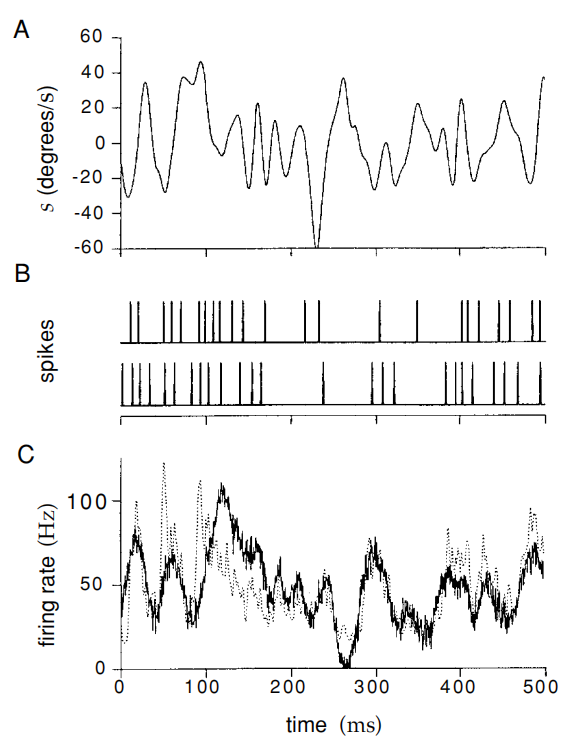
\includegraphics[scale=0.35]{./png/linearFilter}
  \end{center}
\end{exm}

%\subsection{The Most Effective Stimulus}
\begin{defn}
  Neuronal selectivity is often characterized by describing stimuli that evoke maximal responses, subject to a constraint. This stimulus is called the \emph{most effective stimulus}.
\end{defn}

\begin{rem}
  A constraint is essential because the linear estimate in Equation \ref{equ:2.1} is unbounded.
\end{rem}

\begin{defn}
  \label{def:stimulusEnergy}
  The \emph{fixed energy constraint} is
  \begin{equation}
    \label{equ:2.60}
    \int_0^T\left(s(t')\right)^2dt' = constant,
  \end{equation}
  where the integral $\int_0^T\left(s(t')\right)^2dt'$ is called \emph{stimulus energy}.
\end{defn}

\begin{prop}
  \label{prop:mostEffectiveStimulus}
  With the optimal kernel $D(\tau)$ and the fixed energy constraint \ref{equ:2.60}, the most effective stimulus $s(t)$ is proportional to the optimal kernel $D(\tau)$ with
  \begin{equation}
    \label{equ:2.62}
    D(\tau) = -2\lambda s(t-\tau),
  \end{equation}
  where $\lambda < 0$. 
\end{prop}
\begin{proof}
  We impose this constraint by the method of Lagrange multipliers, which means that we must find the unconstrained maximum value with respect to $s$ of
  \begin{equation}
    \label{equ:2.61}
    \begin{aligned}
      r_{\rm{est}}(t)+\lambda\int_0^Ts^2(t')dt' = r_0&+\int_0^{\infty}D(\tau)s(t-\tau)d\tau \\
      &+ \lambda\int_0^T\left(s(t')\right)^2dt',
    \end{aligned}
  \end{equation}
  where $\lambda$ is the Lagrange multiplier. Setting the derivative of this expression with respect to the function s to 0 (similar with the derivative of $E$ in the solution to the proposition \ref{prop:OptimalLinearKernel}) gives \ref{equ:2.62}.
\end{proof}

\begin{rem}
  The value of $\lambda$ (which is less than $0$) in Equation \ref{equ:2.62} is determined by requiring that condition \ref{equ:2.60} is satisfied, but the precise value is not important for our purposes. The essential result is the proportionality between the optimal stimulus and $D(\tau)$.
\end{rem}

\begin{rem}
  The most effective stimulus analysis provides an intuitive interpretation of the linear rate estimate \ref{equ:2.1}. At fixed stimulus energy, the integral in \ref{equ:2.1} measures the overlap between the actual stimulus and the most effective stimulus. In other words, it indicates how well the actual stimulus matches the most effective stimulus. Mismatches between these two reduce the value of the integral and result in lower predictions for the firing
rate.
\end{rem}

\begin{rem}
  As the Example \ref{exm:flyH1LinearEstimate} shows, the linear rate estimate is a good agreement in regions where the measured rate varies slowly, but the estimate fails to capture high-frequency fluctuations of the firing rate, presumably because of nonlinear effects not captured by the linear kernel. Some such effects can be described by a static nonlinear function or including higher-order terms in a Volterra or Wiener expansion, as discussed below.
\end{rem}

\subsection{ Volterra and Wiener Expansion}
\begin{defn}
  \label{VolterraExpansion}
  The \emph{Volterra expansion} is the functional equivalent of the Taylor series expansion used to generate power series approximations of functions. For the case we are considering, it takes the form
  \begin{equation}
    \label{equ:2.2}
    \begin{aligned}
      r_{\rm{est}}(t) = &r_0 + \int D(\tau)s(t-\tau)d\tau \\
      &+ \iint D_2(\tau_1,\tau_2)s(t-\tau_1)s(t-\tau_2)d\tau_1d\tau_2 \\
      &+ \iiint D_3(\tau_1,\tau_2,\tau_3)s(t-\tau_1)s(t-\tau_2)s(t-\tau3)d\tau_1d\tau_2d\tau_3 \\
      &+ \dots.
    \end{aligned}
  \end{equation}
\end{defn}

\begin{defn}
  \label{WienerExpansion}
  The series rearranged by Wiener from Equation \ref{equ:2.2} to make the terms easier to compute has the same first two terms of the Volterra expansion, and it is called \emph{Wiener expansion}.
  % The right side of Equation \ref{equ:2.1} is the first two terms of the Wiener expansion.
  And the linear kernel $D$ is called the \emph{first Wiener kernel}.
\end{defn}

\subsection{Static Nonlinearities}
\begin{rem}
  The linear prediction has two obvious problems:
  \begin{enumerate}[(i)]
  \item there is nothing to prevent the predicted firing rate from becoming negative,
  \item the predicted rate does not saturate, but instead increases without bound as the magnitude of the stimulus increases.
  \end{enumerate}
  One way to deal with these and some of the other deficiencies of a linear prediction is to write the firing rate as a background rate plus a nonlinear function of the linearly filtered stimulus.
\end{rem}

\begin{defn}
  \label{def:staticNonlinearity}
  The \emph{estimate with static nonlinearity} is
  \begin{equation}
    \label{equ:2.8}
    r_{\rm{est}}(t) = r_0 + F(L(t)),
  \end{equation}
  where F is an arbitrary function and
  \begin{equation}
    \label{equ:2.7}
    L(t) = \int_0^{\infty}D(\tau)s(t-\tau)d\tau.
  \end{equation}
  F is called a \emph{static nonlinearity} to stress that it is a function of the linear filter value evaluated instantaneously at the time of the rate estimation.
\end{defn}

\begin{exm}
  $F$ can be extracted from data by means of the graphical procedure illustrated in the following figure. First, a linear estimate of the firing rate is computed using the optimal kernel defined by Equation \ref{equ:2.4}. Next, a plot is made of the pairs of points $(L(t),r(t))$ at various times and for various stimuli, where $r(t)$ the actual rate extracted from the data. There will be a certain amount of scatter in this plot due to the inaccuracy of the estimation. $F$ can be extracted by fitting a function to the points on the scatter plot.
  \begin{center}
    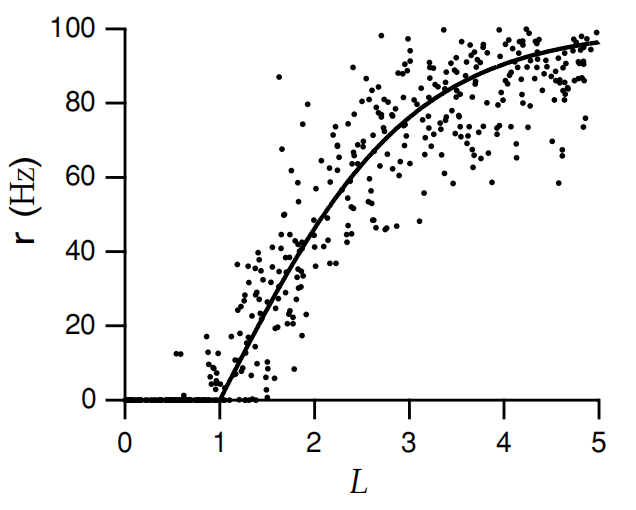
\includegraphics[scale=0.3]{./png/staticNonlinearity}
  \end{center}
\end{exm}

\begin{rem}
  The function $F$ typically contains constants used to set the firing rate to realistic values. These give us the freedom to normalize $D(\tau)$ in some convenient way, correcting for the arbitrary normalization by adjusting the parameters within $F$.
\end{rem}

\begin{exm}
  \label{thresholdFunction}
  The \emph{threshold function}
  \begin{equation}
    \label{equ:2.9}
    F(L) = G[L-L_0]_+,
  \end{equation}
  is a static nonlinearity used to introduce firing thresholds into estimates of neural responses. Here $L_0$ is the threshold value that $L$ must attain before firing begins.
\end{exm}

\begin{rem}
  Above the threshold, the firing rate is a linear function of L, with G acting as the constant of proportionality. Half-wave rectification is a special case of this with $L_0 = 0$. That this function does not saturate is not a problem if large stimulus values are avoided.
\end{rem}

\begin{exm}
  \label{sigmoidalFunction}
  The \emph{sigmoidal function}
  \begin{equation}
    \label{equ:2.10}
    F(L) = \frac{r_{\max}}{1+\exp\left(g_1(L_{1/2}-L)\right)},
  \end{equation}
  is a static nonlinearity used to introduce saturation into estimates of neural responses. Here $r_{\max}$ is the maximum possible firing rate, $L_{1/2}$ is the value of $L$ for which $F$ achieves half of this maximal value, and $g_1$ determines how rapidly the firing rate increases as a function of $L$.
\end{exm}

\begin{exm}
  \begin{equation}
    \label{equ:2.11}
    F(L) = r_{\max}[\tanh(g_2(L-L_0))]_+
  \end{equation}
  is a static nonlinearity that combines a hard threshold with saturation uses a rectified hyperbolic tangent function. Here $r_{\max}$ and $g_2$ play similar roles as in Equation \ref{equ:2.10}, and $L_0$ is the threshold.
\end{exm}

%The following figure shows the different nonlinear functions that we have discussed.
\begin{center}
  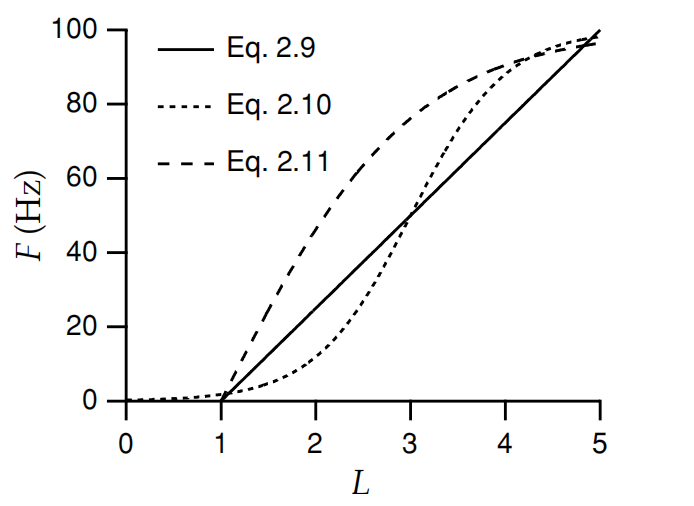
\includegraphics[scale=0.2]{./png/NonlinearExample}
\end{center}

\begin{rem}
  Although the static nonlinearity can be any function, the estimate of Equation \ref{equ:2.8} is still restrictive because it allows for no dependence on weighted autocorrelations of the stimulus or other higher-order terms in the Volterra series.
\end{rem}

\begin{rem}
  Once the static nonlinearity is introduced, the linear kernel derived from Equation \ref{equ:2.4} is no longer optimal because it was chosen to minimize the squared error of the linear estimate $r_{\rm{est}}(t) = r_0 + L(t)$, not the estimate with the static nonlinearity $r_{\rm{est}}(t) = r_0 + F(L(t))$.
\end{rem}

\begin{defn}
  \label{selfConsistency}
  The \emph{self-consistency condition} is that when the nonlinear estimate $r_{\rm{est}}(t) = r_0 + F(L(t))$ is substituted into Equation \ref{equ:2.6}, the relationship between the linear kernel and the firing rate-stimulus correlation function should still hold. In other words, we require that
  \begin{equation}
    \label{equ:2.63}
    D(\tau)  = \frac{1}{\sigma_s^2T}\int_0^Tr_{\rm{est}}(t)s(\tau-t)dt = \frac{1}{\sigma_s^2T}\int_0^TF(L(t))s(\tau-t)dt,
  \end{equation}
  where the second step follows from Assumption \ref{asm:stimulus}.
\end{defn}

\begin{thm}[Bussgang Theorem]
  \label{thm:Bussgang}
  An estimate based on the optimal kernel for linear estimation can still be self-consistent (although not necessarily optimal) when nonlinearities are present, if the stimulus used to extract the optimal kernel is Gaussian white noise.
\end{thm}
\begin{proof}
  If stimulus used to extract $D$ is Gaussian white noise, we have
  \begin{equation}
    \label{equ:2.64}
    \frac{1}{\sigma_s^2T}\int_0^TF(L(t))s(\tau-t)dt = \frac{D(\tau)}{T}\int_0^T\frac{dF(L(t))}{dL}dt.
  \end{equation}
  For the right side of this equation to be $D(\tau)$, the remaining expression must be equal to 1 by appropriate scaling of $F$. The critical identity \ref{equ:2.64} is based on integration by parts for a Gaussian weighted integral.
\end{proof}

\begin{rem}
  The Bussgang Theorem suggests that Equation \ref{equ:2.6} will provide a reasonable kernel, even in the presence of a static nonlinearity, if the white noise stimulus used is Gaussian.
\end{rem}

\begin{exm}
  A model of the spike trains evoked by a stimulus can be constructed by using the firing-rate estimate of Equation \ref{equ:2.8} to drive a Poisson spike generator (see chapter \ref{cha:Neural Encoding I}). The following figure shows the structure of such a model with a linear filter, a static nonlinearity, and a stochastic spike generator.
  \begin{center}
    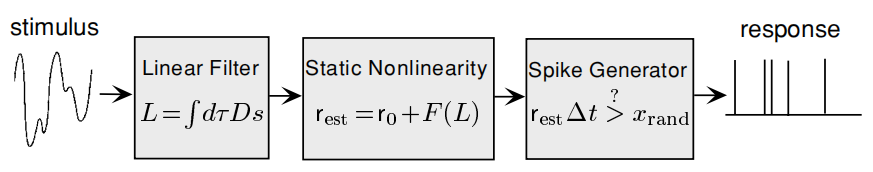
\includegraphics[scale=0.3]{./png/nonlinearGenerator}
  \end{center}
\end{exm}


\begin{rem}
  In some cases, the linear term fails to predict even when static nonlinearities are included and in practice including more terms in the Volterra series is quite difficult to go beyond the first few terms. We can replace the parameter $s$ in Equation \ref{equ:2.7} with an appropriately chosen function of $s$ to improve the accuracy, that is,
  \begin{equation}
    \label{equ:2.12}
    L(t) = \int_0^{\infty}D(\tau)f(s(t-\tau))d\tau.
  \end{equation}
  A reasonable choice for this function is the response tuning curve.
  For time-dependent stimuli, we can think of Equation \ref{equ:2.12} as a dynamic extension of the response tuning curve.
\end{rem}




 









%%% Local Variables:
%%% mode: latex
%%% TeX-master: "../notesOnFluidMechanics"
%%% End:
